\input{D:/Physics/Program/Book-begin.tex}
\usepackage{ctex}

\title{\textbf{Documentation for GEONU Software}}
\author{Shuai Ouyang \thanks{Shuai.Ouyang@snolab.ca}}
\date{2025.03.21}

\begin{document}
	\pdfbookmark{Book Cover}{title} 	%创建封面pdf标签;第一个{}参数是pdf标签的名字,第二个{}参数用于hyperlink,
	\maketitle							%显示封面
	\thispagestyle{empty}				%封面取消页码
	\frontmatter						%页码使用罗马字母
	\cleardoublepage				 	%消除一张空白页,为了在pdf中实现目录的跳转
	\pdfbookmark{\contentsname}{toc} 	%创建目录pdf标签
	\tableofcontents				  	%生成目录
	\mainmatter							%页码使用拉丁数
	\chapter{Introduction}
		\section{什么是地球中微子}
			简单来说,Geonu指的是来自地球内部的中微子。这个课题的研究来自于地质学,早先地质学家通过地震波研究清楚了地球的内部结构,对地球内部的物理性质了解的十分清楚,但对化学性质却知之甚少。地球的化学性质对于地球的演化非常重要,例如地球表面的大陆板块运动、地幔的物质循环就十分依赖地球内部化学性质。目前也有不少能够描述地球内部化学性质的理论,但是人类的地下活动仅仅$12$ km,并没有多少关于地幔的直接测量数据,所以需要实验来辨别哪些理论是正确的,哪些理论是错误的。\par
			推动地球内部运动的能量来源一部分来自于元素的衰变,这些元素统一被称作HPE。地质学家注意到HPE衰变,例如${}^{235}U, {}^{238}U, {}^{232}Th, {}^{40}K$,在产生热量的同时会释放中微子\cite{fiorentini2007geo} (Eq.\ref{Decay:U235}-\ref{Decay:K40_2});由于中微子只参与弱相互作用,所以它可以很轻易地将地球内部的信息传递出来,所以地球中微子成为了人类认识地球内部化学性质的一个重要手段。
				\begin{align}
					&{}^{235}U \longrightarrow {}^{207}Pb + {}^{4}He + 4e^- + 4\overline{\nu}_e + 0.283 \text{ MeV},
					\label{Decay:U235}\\
					&{}^{238}U \longrightarrow {}^{206}Pb + 8\alpha + 6e^- + 6\overline{\nu}_e + 51.7 \text{ MeV},
					\label{Decay:U238}\\
					&{}^{232}Th \longrightarrow {}^{208}Pb + 6\alpha + 4e^- + 4\overline{\nu}_e + 42.7 \text{ MeV},
					\label{Decay:Th232}\\
					&{}^{40}K \longrightarrow {}^{40}Ca + e^- + \overline{\nu}_e + 1.31 \text{ MeV} \,(89.3\%),
					\label{Decay:K40_1}\\
					&{}^{40}K \longrightarrow {}^{40}Ar + \nu_e + 1.505 \text{ MeV} \,(10.7\%).
					\label{Decay:K40_2}
				\end{align}
			目前探测地球中微子的方式是通过IBD反应:
				\begin{equation}
					\overline{\nu}_e + p \longrightarrow n + e^+,
				\end{equation}
			正电子迅速与电子湮灭,在实验上产生promt信号;中子之后随机游走,并且在游走的过程中能量逐渐降低,最终被质子俘获从而在实验上产生delayed信号。由于这个反应的阈值为$1.806$ MeV,目前人类只能看到来自${}^{238}U$和${}^{232}Th$衰变的地球中微子(Fig.\ref{Fig:Geonu Decay})。
				\begin{figure}[H]
					\centering
					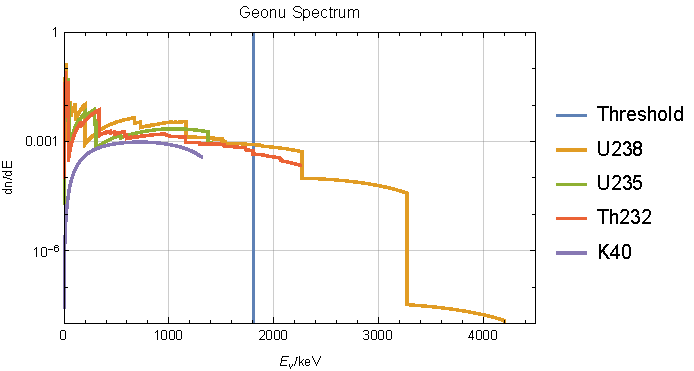
\includegraphics[scale = 1.2]{./Pics/Geonu_Decay_Spectrum.pdf}
					\caption{不同HPE元素衰变的地球中微子能谱\cite{Enomoto_Spectrum}}
					\label{Fig:Geonu Decay}
				\end{figure}
		\section{GEONU Software}
			GEONU是一款开源的MATLAB代码,目前有Tytrice Faison和Laura Sammon负责维护\cite{Original_GEONU},这款软件对地球进行建模并且能够计算各个探测器的地球中微子信号,除此之外还有geonu flux、热功率等信息。我在此基础上对整套代码进行了改写,提高了可读性、可维护性,做到了模块化,以便于后续SNO+对地球中微子问题的研究。\par
			GEONU将地球划分成三大部分:Lithsophere、Mantle和Core;由于Core对地球中微子信号几乎没有贡献,所以着重计算了来自Lithosphre和Mantle的信号。Lithosphere被划分成了7层,分别是sediment(s1, s2, s3), Crust(UC, MC, LC)和LM,每一层按照经纬度划分成了$1^\circ \times 1^\circ$的cell,总共$64,800$个格子,如Fig. \ref{Fig:Earth Structure 1}。Mantle部分则是划分成了两层,分别是DM和EM,每一层同样是$64,800$个格子。整体结构看见Fig. \ref{Fig:Earth Structure 2}
				\begin{figure}[H]
					\centering
					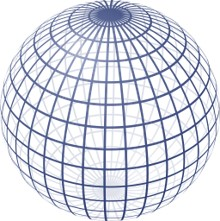
\includegraphics[scale = 1]{./Pics/Earth_Structure_1.jpg}
					\caption{地层划分演示}
					\label{Fig:Earth Structure 1}
					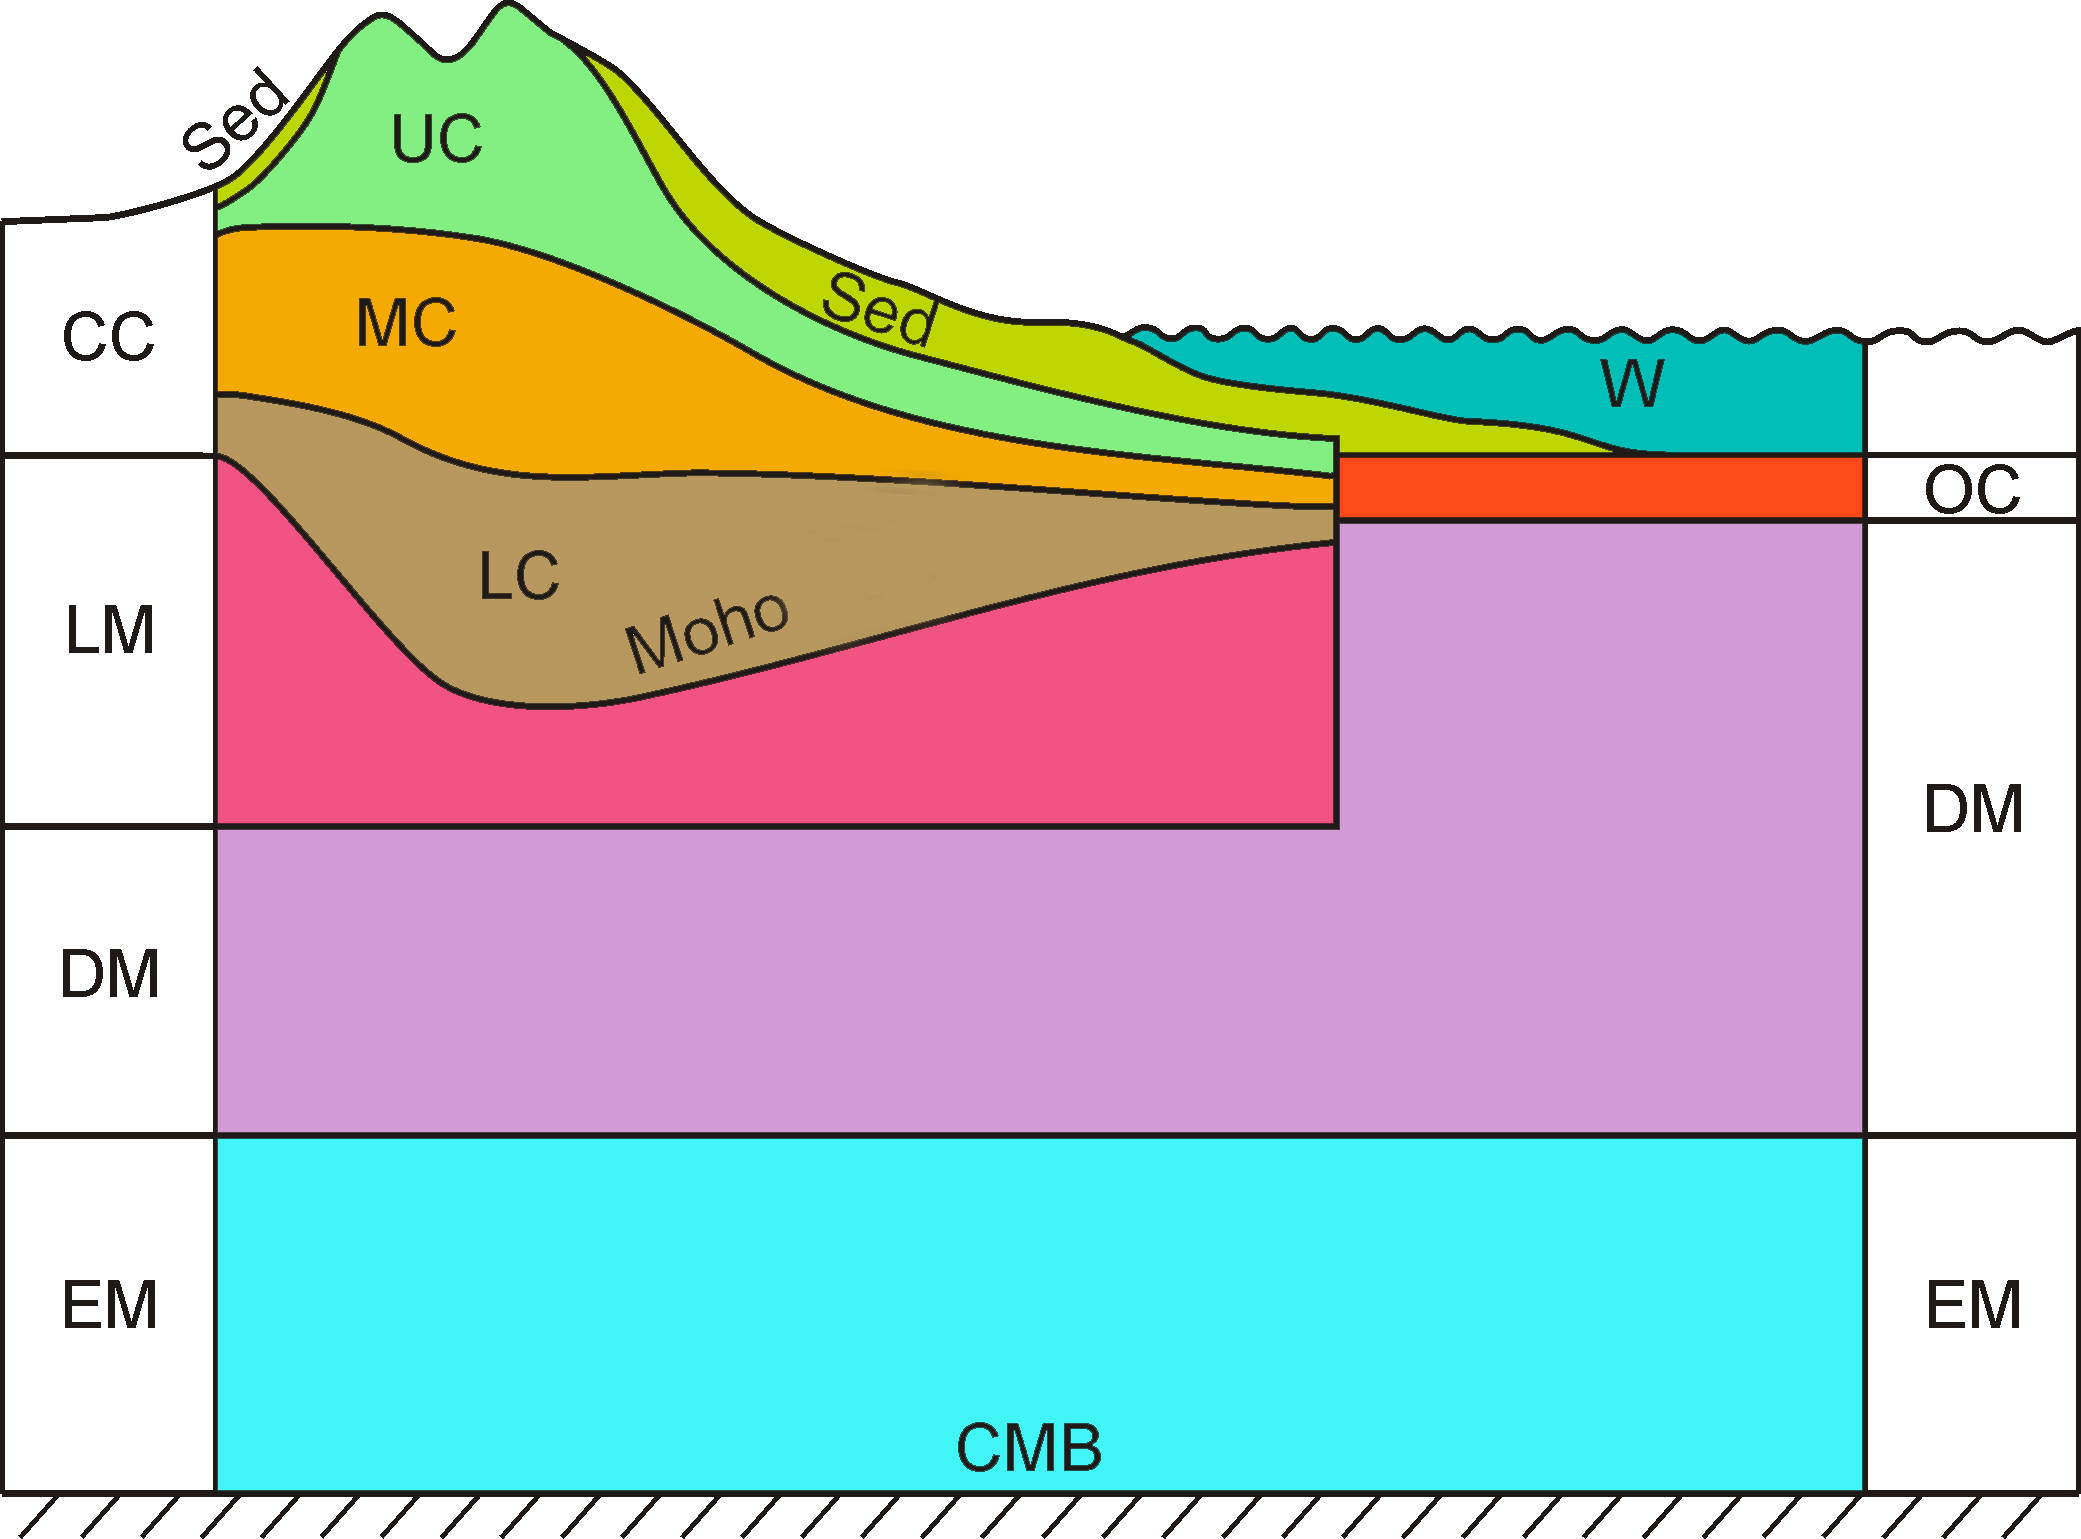
\includegraphics[scale = 0.15]{./Pics/Earth_Structure_2.jpg}
					\caption{地球内部结构\cite{huang2013reference}}
					\label{Fig:Earth Structure 2}
				\end{figure}
			除此之外,GEONU输入了不同的地质模型数据。Lithosphere可选择数据有Crust1.0, Crust2.0, Lith和ECM;Mantle导入的数据是PREM。目前,整个改写工作Lithosphere只支持Crust1.0模型。\par
			有了地球建模之后,接下来就是如何计算地球中微子信号。对于第$i$的HPE元素,其产生的信号为
				\begin{equation}
					S_i
					= \int_{\oplus} \rho A_i dV \times \frac{1}{a_i} \times \frac{\ln 2}{\tau_i}\times \int \frac{dn}{dE} \sigma_{IBD} dE \times \frac{P_{ee}}{4\pi L^2} \times 1 \text{yr} \times N_{proton} \times \varepsilon_{detector},
				\end{equation}
			where $\rho$ is rock density; $A_i$ is abundance of i-th HPE; $N_{avg}$ is Avogadro constant; $a_i$ is atom mass; $\tau_i$ is half-life ot i-th HPE; $P_{ee}$ is survival probability; $L$ is distance from rock to detector; $N_{proton}$ is the number of proton; $\varepsilon_{detector}$ is detection efficiency.\par
			至此,整个GEONU计算框架到此结束,更加详细的细节和讨论将会放到后续章节当中。
		\section{How to use GEONU Software?}
			如果你是第一次接触、使用GEONU软件的话,请首先安装MATLAB软件。安装完成之后,打开\textbf{main.mlx}文件,选择你关注的探测器,设置想要的迭代次数,然后点击程序运行。迭代次数和内存息息相关,请参考下列的推荐表格:
				\begin{table}[H]
					\centering
					\caption{Recommendation for iteration}
					\begin{tabular}{|c|c|c|}
						\hline
						Iteration & Recommended Memory & Cost Time\\
						\hline
						$1000$ & $32$ GB & $102$ s\\
						\hline
						$4000$ & $64$ GB & $280$ s\\
						\hline
					\end{tabular}
				\end{table}
			程序结束之后,结果会保存在\textbf{Output}文件夹。计算结果保存了三个structure:Physics、Geology和Output。前两个记录物理和地质输入,以便于后续检查和复现;Output记录计算结果。\textbf{Plot.m}文件展示了如何读取、展示计算结果,所有输出图片都会保存在\textbf{Pics}文件夹当中。
	\chapter{Input Parameters}
	\chapter{Software Design}
	\bibliographystyle{unsrt}			
	\bibliography{ref}					%调用文献bib,注意bib文件名和路径名全部不能有空格;用\cite引用文献
	\addcontentsline{toc}{chapter}{Reference} %PDF中增加Reference的跳转
\end{document}